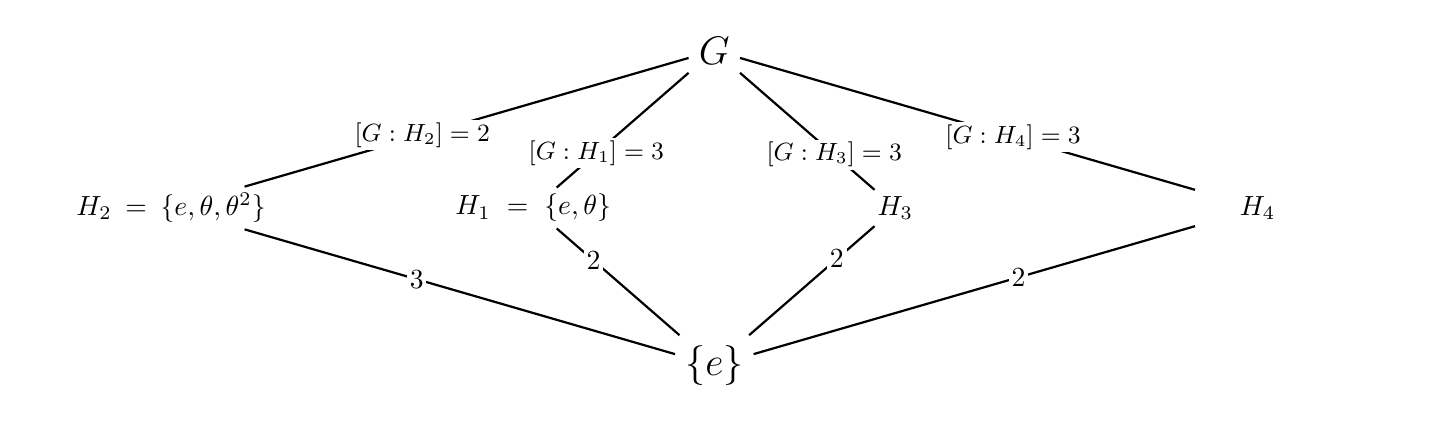
\begin{tikzpicture}[
		thick,
		xscale=1.15,
		% Definimos un estilo para los nodos:
		% text width=3.5cm: Forzamos a que todos tengan el ancho del más grande (H2)
		% align=center: Centramos el texto dentro de esa caja invisible
		myNode/.style={text width=3.5cm, align=center, inner sep=2pt}
	]

	% --- 1. Definición de Nodos ---
	% Usamos coordenadas simétricas (-6, -2, 2, 6)

	\node (G) at (0, 4) {\Large $G$};

	% Al usar el estilo 'myNode', cada etiqueta se centra en su propia "caja" de 3.5cm
	% Esto asegura que las líneas conecten exactamente al centro geométrico.
	\node[myNode] (H2) at (-6, 2) {$H_2=\{e, \theta, \theta^2\}$};
	\node[myNode] (H1) at (-2, 2) {$H_1=\{e, \theta\}$};
	\node[myNode] (H3) at (2, 2)  {$H_3$};
	\node[myNode] (H4) at (6, 2)  {$H_4$};

	\node (e) at (0, 0) {\Large $\{e\}$};

	% --- 2. Conexiones Superiores ---
	% Ajustamos las posiciones (pos) para escalonar las etiquetas y que no choquen

	\draw (G) -- node[fill=white, inner sep=1pt, pos=0.6] {\small $[G:H_2]=2$} (H2);
	\draw (G) -- node[fill=white, inner sep=1pt, pos=0.7] {\small $[G:H_1]=3$} (H1);
	\draw (G) -- node[fill=white, inner sep=1pt, pos=0.7] {\small $[G:H_3]=3$} (H3);
	\draw (G) -- node[fill=white, inner sep=1pt, pos=0.6] {\small $[G:H_4]=3$} (H4);

	% --- 3. Conexiones Inferiores ---
	\draw (H2) -- node[fill=white, inner sep=1pt, pos=0.4] {3} (e);
	\draw (H1) -- node[fill=white, inner sep=1pt, pos=0.3] {2} (e);
	\draw (H3) -- node[fill=white, inner sep=1pt, pos=0.3] {2} (e);
	\draw (H4) -- node[fill=white, inner sep=1pt, pos=0.4] {2} (e);

\end{tikzpicture}
